
\newpage
\hfill\par
\hfill\par
\centerline{\Huge\textbf iOS}\par
\hfill\par
\hfill\par
Apps no iOS estão isoladas umas das outras através de uma sandbox(Seatbelt) cujo propósito é limitar os danos ao sistema e aos dados do utilizador caso a aplicação seja corrompida. Existe também um controlo de acesso mandatorio (MAC) que descreve os recursos que a aplicação pode usar.\par

Oferece poucos CIP(comunicação inter-processos) o que minimiza os vetores de ataque.

\section{Aspetos de Segurança do iOS}

\subsection{Secure Boot}
\hfill\par

		Quando Um dispositivo iOS é ligado começa por ler as instruções de uma memória read-only conhecida com Boot ROM.
		Esta garante que a assinatura do Low Level Bootloader está correta e o Low Level Boot Loader faz o mesmo com o iBoot bootloader, que por sua vez verifica a assinatura do iOS Kernel.\par
		Se o Boot ROM falhar, o dispositivo entra no modo Device Firmware Upgrade (DFU)\footnote[1]{DFU or Device Firmware Upgrade mode permite que um dispositivo tenha o seu software restaurado independentemente do estado em que se encontre.}, se algum dos outros passos falhar o dispositivo entra em modo de recuperação.


\subsection{File System Encryption}
\hfill\par
	Cada dispositivo iOS tem 2 chaves AES de 256 bits (User ID e Group ID) que são guardadas no processador de aplicações durante o fabrico. Apenas os crypto-engines tem acesso ás chaves e o User ID é usado para garantir a encriptação dos ficheiros dentro do iOS.\par
	Como os UIDs não são guardados no fabrico, nem a Apple pode restaurar as chaves de encriptação de um dispositivo\footnote[2]{Isto acontece porque a chave está gravada no chip de silicone}.\par


\subsection{ Code Signing}
\hfill\par
	Não é possivel correr código num iOS que não seja jailbroken\footnote[3]{telemoveis "Jailbroken" são telemoveis modificado para fornecer acesso a todo o sistema de ficheiros\cite{ref_intro2}} a não ser que a Apple o permita. Para correr uma aplicação é preciso um perfil de desenvolvedor e um certificado assinado pela Apple.


\subsection{ App Store Data Protection}
\hfill\par
	Quando se decarregam aplicações da App Store é aplicado o FairPlay Code Encryption sobre estas. O processo para a implementação desta encriptação segue os seguintes passos:\par
	\begin{enumerate}
	\item Quando se regista uma nova conta Apple um par de chaves publica/privada é criada e atribuida à conta sendo que a privada é armazenada no dispositivo iOS e a pública fica na App Store.\par
	\item Quando se quer descarregar uma aplicação, a App Store encripta com a chave pública a mesma e o dispositivo quando quiser usar a aplicação pela primeira vez após ser ligado desencripta-a com a chave privada\footnote[3]{Cada dispositivo tem um crypto-engine dedicado que fornece a geração de uma chave AES de 256 bit e um hash SHA-1.}.\par
\end{enumerate}

\subsection{ General Exploit Mitigations}
\hfill\par
	Sempre que um aplicação é executada a alocação da memória para a aplicação é aleatória prevenindo ataques de injeção de código.\par
	As bibliotecas a usar pelas aplicação, como são comuns, são alocadas aleatóriamente quando o dispositivo é ligado e não sempre que uma aplicação que as requer é iniciada.\par
\hfill\par
\hfill\par
Apesar de todos os mecanismos de segurança implementados ainda podem ser encontrados problemas em:
\renewcommand{\theenumi}{\Roman{enumi}}
\begin{enumerate}
	\item Proteção de dados na memória.
	\item Keychain.
	\item Touch ID.
	\item dados na rede.
\end{enumerate}
\renewcommand{\theenumi}{\arabic{enumi}}


\section{iOS Application Attack surface}
\hfill\par

Uma aplicação iOS pode estar vulneráve a ataques caso não:

\renewcommand\labelitemi{.}
\begin{itemize}

\item Valide todos os inputs através de uma comunicação IPC ou esquema URL.

\item Valide todos os inputs que o utilizador insira nos campos que preenche.

\item Valide o conteudo carregado dento de uma página web.

\item Comunique de forma segura com os servidores que prestam serviços ou seja suscetivel a ataques man-in-the-middle.

\item Guarde de forma segura os dados locais ou carregue dados de terceiros suspeitos.

\item Tenha proteção contra ambientes comprometidos, reempacotamento ou outros ataques\cite{ref_intro3}. 


\end{itemize}

\section{TESTES DE SEGURANÇA EM APLICAÇÕES}
\hfill\par

\subsection{Data Storage on iOS}
\hfill\par
A proteção de dados sensíveis como tokens de autenticação e dados privados é uma chave para a segurança no telemovel.


\subsubsection{Testar o Armazenamento Local (MSTG-STORAGE-1 and MSTG-STORAGE-2)}
\hfill\par
\hfill\par


  Secure Enclave Processor (SEP):\par

\begin{figure}[H]
\centering
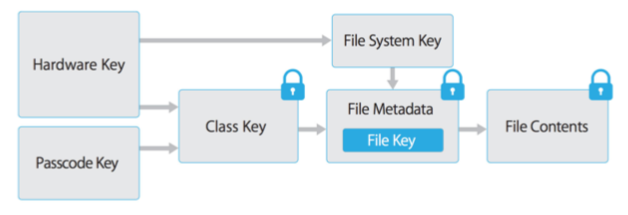
\includegraphics[width=\textwidth]{image17.png}
\caption {Secure Enclave Processor Scheme}
\label {fig01}
\end{figure}

 		A arquitetura é baseada numa hierarquia de chaves.
 		O User ID e uma passcode key que é derivada da aplicação do algoritmo PBKDF2 sobre a password de desbloqueio do dispositivo. 
 		Classkey está associada ao estado do dispositivo (bloqueado ou desbloqueado).
 		Cada ficheiro guardado no sistema de ficheiros está encriptado com uma chave por ficheiro.\par


Ficheiros têm 4 tipos de classes de proteção:

\begin{itemize}
\item \textit{Proteção completa:}
		A chave de classe é apagada da memória após o dispositivo ser bloqueado.Tornando os dados inacessiveis quando o dispositivo está bloquado.\par
		\hfill\par

\item \textit{Proteção até ser aberta:}
		Igual à anterior mas a chave não é apagada quando o dispositivo é bloqueado permitindo acesso ainda bloqueado. Útil para emails.\par
		\hfill\par
\item \textit{Proteçã até primeira autenticação do utilizador:}
		O ficheiro pode ser acedido mal o utilizador desbloqueie o dispositivo após liga-lo.\par
		\hfill\par
\item \textit{Sem proteção:}
		A chave de classe é guardado na \textit{Effaceable Storage\footnote[0]{A \textit{Effaceable Storage} é uma flash memory para pequenos dados que nunca é apagada.}}\par
\end{itemize}


Para realizarmos o teste ao armazenamento local, de forma a verificarmos se conseguimos aceder ao conteúdo dos dados basta seguirmos estes passos.

\begin{enumerate}
\item Acionar a funcionalidade da aplicação que guarda dados sensíveis, por exemplo fazer login na aplicação.

\item navegar até à diretoria com os ficheiros sensíveis.
\begin{lstlisting}
/var/mobile/Containers/Data/Application/$APP_ID/
\end{lstlisting}
\item executar grep com os dados guardados por exemplo: \textit{grep -iRn <USERID>}.

\end{enumerate}

Se os dados forem legiveis o teste falhou.


\subsubsection{Determinar se dados sensíveis são enviados para terçeiros (MSTG-STORAGE-4)}
\hfill\par
\hfill\par
Regras:
\begin{itemize}
\item Não deve ser enviada mais informação do que a estritamente necessária.
\item Todos os dados enviados para terceiros deve ser anonimizado para impedir exposição de PII (	Personal Identifiable Information).
\end{itemize}
Para realizar este teste basta usar um proxy para podermos intercetar o tráfico entre a aplicação e os terçeiros. Posteriormente podemos analisar o tráfico e se estiver a ser enviada informação sensivel pessoal, o teste falha.



\subsubsection{Procurar dados sensíveis na cache do teclado (MSTG-STORAGE-5)}
\hfill\par
\hfill\par

   O protocolo UITextInputTraits é usado para a cache do teclado e possui 2 propriedades: 
\begin{itemize}

   		\item \textit{var autocorrectionType UITextAutocorrectionType:} 

   			Determina se a correção automática está ativada durante a escrita, o valor por defeito desta propriedade é UITextAutocorrectionTypeDefault, que permite autocorreção. \par
   			\hfill\par

   		\item \textit{var secureTextEntry:}

   			Variável responsável por definir se se mantêm as palavras escritas em cache e se se escondem as palavras escritas nos campos UITextField. Por defito é NO.
\end{itemize}


   	O objetivo deste teste é procurar no código fonte da aplicação uma implementação semelhante à da figura para os UITextFields visados. Se estes não tiverem a configuração mostrada falham o teste.

\begin{figure}[H]
\centering
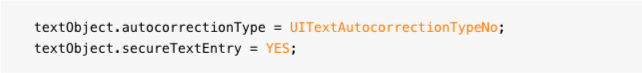
\includegraphics[width=\textwidth]{image26.png}
\caption {Secure Text Entry Example}
\label {fig02}
\end{figure}



Para corrigir este problema podemos programar uma solução para o UITextField alvo apicando o código: \textit{textObject.autocorrectionType = UITextAutocorrectionTypeNo} aos \textit{UITextFields}, \textit{UITextViews} e \textit{UISearchBars} que desejarmos. Para objetos que devem ser mascarados devemos definir o atributo \textit{textObject.secureTextEntry} como \textit{YES}.  Na imagem abaixo vemos um exemplo.
	 
\begin{figure}[H]
\centering
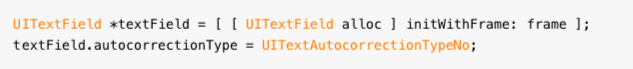
\includegraphics[width=\textwidth]{image27.png}
\caption {Set a secure Text Entry}
\label {fig02}
\end{figure}

Para testar se a cache do teclado possui dados sensiveis que não deveriam ser guardados, basta:
\begin{enumerate}
	\item Fazer reset à cache do teclado.
	\item Entrar na aplicação e inserir, por exemplo, os dados de autenticação.
	\item Sair da aplicação.
	\item Reentrar na aplicação e começar a reinserir os dados. 
	\item Se for permitido completar automáticamente o preenchimento dos dados, o teste falha.
\end{enumerate}



\subsubsection{Procurar exposição de dados sensíveis na interface do utilizador (MSTG-STORAGE-7)}
\hfill\par
\hfill\par


A inserção de informação sensível é necessária quando queremos por exemplo levantar dinheiro, fazer um pagamento entre outros. Ao utilizar aplicações que requerem esse tipo de dados sensíveis é imperativo que estes não sejam mostrados em texto limpo na interface após inseridos.\par
\hfill\par
Um campo que mascare o que nele é escrito pode ser verificado de duas formas.
A primeira pode ser verificada navegando pelo código da aplicação até à configuração da caixa que recebe os dadso sensíveis e verificando se a opção \textit{Secure Text Entry} está ativa, se estiver ativa o texto inserido é substituido por pontos.
A segunda é em interação com a aplicação a testar inserir os dados sensiveis e verificar se os dados aparecem em texto limpo ou são mascarados.



\subsection{iOS Cryptographic APIs}

\hfill\par

\subsubsection{Verificação da configuração dos algoritmos criptográficos standard (MSTG-CRYPTO-2 and MSTG- CRYPTO-3)}
\hfill\par
\hfill\par

O CriptoKit da Apple tem os seguintes algoritmos:
\begin{itemize}
\item \textit{Hashes:}

\begin{figure}[H]
\centering
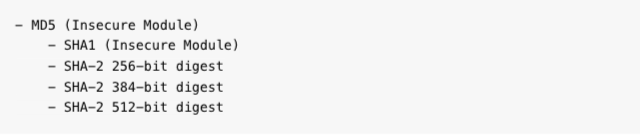
\includegraphics[width=\textwidth]{image38.png}
\caption {Available Hash Algorithms}
\label {fig02}
\end{figure}

\item \textit{Symmetric-Key:}

\begin{figure}[H]
\centering
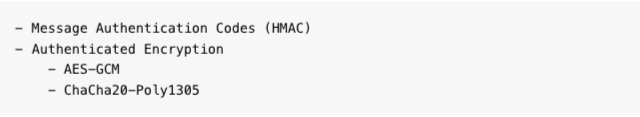
\includegraphics[width=\textwidth]{image39.png}
\caption {Available Symmetric-key Algorithms}
\label {fig02}
\end{figure}
\item \textit{Public-Key:}

\begin{figure}[H]
\centering
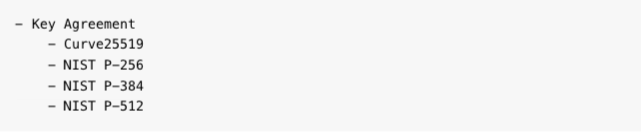
\includegraphics[width=\textwidth]{image40.png}
\caption {Available Public-key Algorithms}
\label {fig02}
\end{figure}
\end{itemize}

Se a aplicação usar implementações fornecidas no kit, a melhor forma de verificar o estado do algoritmo é analizando as chamadas ás funções do CommonCryptor. 

\begin{figure}[H]
\centering
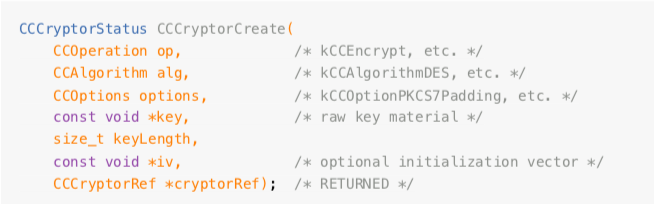
\includegraphics[width=\textwidth]{image41.png}
\caption {CommonCryptor Status}
\label {fig02}
\end{figure}

Podemos depois comparar os enums para determinar o algoritmo, o padding e a chave usados.
Após determinarmos os 3 podemos verificar se estes são seguros ou se já estão ultrapassados.



\subsubsection{Testar Gestão de Chaves (MSTG-CRYPTO-1 and MSTG-CRYPTO-5)}
\hfill\par
\hfill\par
Quando guardamos uma chave é recomendado o uso do keyChain desde que não se use o atributo kSecAttrAccessibleAlways.

O mecanismo de keyChain permite 2 formas de guardar chaves:
\begin{enumerate}
	\item Usar uma chave de segurança guardada no secure-enclave para encriptar a chave.

	\item Guardar a chave no secure-enclave\footnote[4]{ O Secure-enclave é um gestor de chaves baseado em hardware e isolado do processador para maior segurança\cite{book}.}.
\end{enumerate}



O teste tem de ser monitorizado verificando o acesso aos ficheiros do sistema durante operações criptográficas da aplicação.

O teste falha se:

	- Chaves usadas para proteger dados sensíveis são sincronizadas entre dispositivos.

	- Chaves não são guardadas com proteção.

	- Chaves não são derivadas de funcionalidades estáveis do dispositivo.

	- Chaves não são escondidas ao usar linguagens de baixo nivel.

	- Chaves são importadas de locais inseguros.




\subsubsection{Testar Geração Aleatória de Números (MSTG- CRYPTO-6)}
\hfill\par
\hfill\par

A Apple fornece uma API para gerar números aleatório criptográficamente seguros.

Em Swift a chamada à API é feita com o seguinte código:

\begin{lstlisting}[basicstyle=\small,]
    func SecRandomCopyBytes(_ rnd: SecRandomRef?,
                      _ count: Int,
                      _ bytes: UnsafeMutablePointer<UInt8>) -> Int32
\end{lstlisting}

 
A versão em Objective-C é:
\begin{lstlisting}[basicstyle=\small,]
 int SecRandomCopyBytes(SecRandomRef rnd, size_t count, uint8_t *bytes);
\end{lstlisting}
Um exemplo de utilização é:
\begin{lstlisting}[basicstyle=\small,]
  int result = SecRandomCopyBytes(kSecRandomDefault, 16, randomBytes);
\end{lstlisting}

Para testar se a implementação usada é segura basta verificar que a geração de números aleatórios, se não for igual ás acima descritas, sejam wraplicaçãoers implementados sobre a API acima. 

\textit{Nota: Podemos usar o plugin \textbf{Burp's sequencer} para avaliar a qualidade da geração dos números.}


\subsection{Local Authentication on iOS}
\hfill\par
Durante a autenticação local, uma aplicação autentica um utilizador verificando con credenciais guardadas localmente no dispositivo (PIN, password, carateristicas biometricas).

Atacantes podem facilmente passar a autenticação local caso nada seja retornado do processo de autenticação.


\subsubsection{Testar Autenticação Local (MSTG-AUTH-8 and MSTG-STORAGE-11)}
\hfill\par
\hfill\par
É importante lembrar que a framework de autenticação local é um processo baseado em eventos e portanto não deve ser o único método de autenticação.\par
\hfill\par


Apesar de ser uma autenticação eficiente ao nivel do utilizador, esta é facilmente ultrapassável usando instrumentos de patching. Assim é melhor usar o método de serviço da keyChain, ou seja, verificar que processos sensíveis são protegidos com métodos de serviço da keyChain. ex: transações financeiras.\par

Verificar as flags dos controlos de acesso da keyChain para assegurar que os dados só são acedidos pelo utilizador. Podem-se utilizar as seguintes flags: 

\begin{itemize}

\item \textit{kSecAccessControlBiometryCurrentSet:}\par
	\hfill\par
	Esta flag obriga o utilizador a autenticar-se biometricamente antes de aceder à keyChain. Se for adicionado um novo dado biométrico, a entrada na keyChain vai ser invalidada e só poderá ser acedida pelos utilizadores autenticados quando os dados foram adicionados.\par
	\hfill\par

\item \textit{kSecAccessControlBiometryAny:}\par
	\hfill\par
	Esta flag obriga o utilizador a autenticar-se biometricamente antes de aceder à keyChain. Caso novos dados biométricos sejam adicionados a autenticação na keyChain mantem-se. Útil para utilizadores que mudam a própria impressão digital mas bom para atacantes também visto que se conseguirem registar a impresão digital conseguem aceder aos restantes dados biométricos.\par
	\hfill\par

\item \textit{kSecAccessControlUserPresence:}\par
	\hfill\par
	Permite que o utilizador se autentique por password se autenticação biométrica não funcionar. É mais fraco visto ser mai facil roubar uma password por shouldersurfing do que passar pelso dados biométricos.
\end{itemize}

Para garantir que os dados biométricos podem ser usados temos de verificar se a classe kSecAttrAcessibleWhenPasscodeSetThisDeviceOnly ou a kSecAttrAcessibleWhenPasscodeSet estão implementadas\footnote[5]{A variante ThisDeviceOnly garante que não há sincronização dos dados biométricos entre dispositivos iOS.}.\par
\hfill\par

Para um dispositivo \textit{jailbroken} existem ferramentas que permitem efetuar uma quebra na segurança da autenticação local. Neste exemplo usaremos o Swizzler2, uma ferramenta que através do uso do software Frida permite que a função de autenticação retorne True mesmo que tenha falhado.\par
\hfill\par
Os passos para efetuar o teste são:
\begin{enumerate}
\item Ir aos settings e escolher Swizzler
\item Permitir injeção do Swizzler nas aplicações
\item Permitir registar tudo no Syslog
\item Permitir registar tudo num ficheiro
\item Entrar nos submenus da framework iOS
\item Permitir autenticação local
\item Entrar no submenu e escolher as aplicações alvo
\item Permitir que a aplicação escolhida corra
\item Reiniciar a aplicação
\item Quando for pedida a impressão digital carregar em cancelar
\end{enumerate}

Se a aplicação continuar sem requerer a impressão digital esta não passou no teste.



\subsection{iOS Network APIs}
\hfill\par
Quase todas as aplicações no iOS atuam como cliente de um ou mais serviços remotos.  Como não podemos confiar nas redes pública. Temos portanto de garantir que as aplicações tomam medidas para mitigar os riscos. 


\subsubsection{Segurança da Camada de Trasporte da Aplicação (MSTG-NETWORK-2)}
\hfill\par
\hfill\par
 A App Transport Security (ATS) é um conjunto de verificações de segurança que o sistema operativo realiza quando efetua conecções com NSURLConnection\footnote[6]{ Conecções NSURLConnection permitem carregar conteúdos de um URLao fornecer um pedido para um objeto URL\cite{ref_intro4}.}, NSURLSession\footnote[7]{A classe NSURLSession fornece uma API para download e para upload de dados entre pontos opostos de uma conexão indicados por URLs\cite{ref_intro5}.} e CFURL\footnote[8]{ O tipo CFURL fornece facilidade para criar, percorrer e desreferenciar strings URL\cite{ref_intro6}.} a servidores públicos. Estas verificações são efetuadas por defeito do iOS SDK 9 em diante.\par
Quando a ligação é feita a um IP, um dominio de nomes não qualificado ou TLD de .local o ATS não é aplicado.\par
\hfill\par
Agora vamos ver uma análise das configurações da ATS.\par

Se o código fonte estiver disponivel devemos abrir a Info.plist na diretoria da aplicação (\textit{Bundle Directory}) que o desenvolvedor configurou. Na imagem abaixo vemos um exemplo de uma exceção configurada para desativar as restrições globais da ATS.

\begin{figure}[H]
\centering
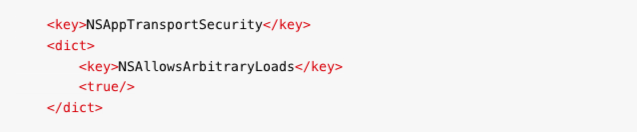
\includegraphics[width=\textwidth]{image42.png}
\caption {ATS example configuration}
\label {fig02}
\end{figure}

A desativação das restrições da ATS depende da aplicação, por exemplo a aplicação do chrome para iOS tem estas configurações, o que é aceitavel visto que por outro lado a aplicação não se conseguiria ligar a um site HTTP que não tivesse todos os requisitos da ATS.

As recomendações para o uso da ATS são:
\begin{itemize}
\item A ATS deve ser configurada de acordo com as melhores práticas aconcelhadas pela Apple e só deve ser desativada excecionalmente.\par
\hfill\par
\item Se a aplicação se conectar a um número definido de dominios que o dono da aplicação controla, esses dominios devem suportar a ATS.\par
\hfill\par
\item Se houver conecções a terçeiros (que não pertençam ao dono da aplicação) devem ser avaliados quais os requisitos da ATS que não são suportados e podem ser desativados.\par
\hfill\par
\item Se a apicação abrir sites web de terçeiros, do iOS 10 para a frente pode-se usar o \textit{NSAllowsArbitraryLoadsInWebContent} para desabilitar as restrições da ATS para o conteúdo das páginas web.
\end{itemize}

\subsubsection{Teste e Validação de Certificados (MSTG-NETWORK-3 and MSTG-NETWORK-4)}
\hfill\par
\hfill\par

As autoridades de cetificação são uma parte fulcral da comunicação cliente-servidor. No iOS existem uma quantidade enorme de certificados confiáveis. CAs podem ser adicionadas manualmente pelo utilizador ou por malware, para precaver esta situação basta  remover a confiança nas CAs adicionadas.\par
Falhas podem ocorrer se a aplicação esperar outra chave ou certificado do servidor, ou pode estar a ocorrer um ataque.
Nestes casos basta seguir os passos referidos no capitulo \textit{Android Network APIs}\cite{book}.\par
\hfill\par
Em baixo apresentamos 3 formas de manter os certificados confiaveis por parte da aplicação.
\begin{enumerate}
\item Incluir os certificados do servidor na diretoria da aplicação e verifica-lo a cada conecção. Isto requer um mecanismo de atualização do certificado para o caso do certificado mudar.\par
\hfill\par
\item Limitar os emissores de certificados, ex: uma CA envia à aplicação o certificado de um servidor. O certificado será seguro e limita ataques possíveis.\par
\hfill\par
\item A aplicação deve possuir a chave pública da CA confiavel pertencente ao dono da aplicação. Isto não requer atualizar a aplicação sempre que o servidor mudar de certificado. Usar uma CA própria faz com que o seu certificado seja auto assinado.
\end{enumerate}

Para validarmos os certificados presentes na aplicação vamos usar o Burp para intercetar o tráfico que circula entre a aplicação a testar e o seridor a que esta se está a ligar. Posteriormente realizamos os seguintes passos pela ordem em que aparecem.

\begin{enumerate}
\item Temos de verificar se ferramentas como o SSL Kill Switch estão desativadas.\par
\hfill\par
\item Garantir que não há certificados a serem adicionados à diretoria da aplicação.\par
\hfill\par
\item Iniciar a aplicação, se conseguirmos ver o tráfico não é realizada nenhuma validação do certificado e a aplicação falhou o teste.\par
\hfill\par
\item Se houver uma falha no SSL handshake (está a ser verificada a validade do certificado), instalamos o certificado do  Burp.\par
\hfill\par
\item Se o handshake for bem sucedido e conseguimos ver o tráfico, o certificado foi validado com o certificado na diretoria da aplicação mas não pela cadeia de confiança da mesma. A aplicação falha neste ponto se tal ocorrer.
\end{enumerate}


Se não conseguirmos ver o tráfico apesar do SSL handshake funcionar então todas as medidas de segurança para o establecimento da conecção foram tomadas e a aplicação passou no teste.


\subsection{iOS Platform APIs}
\hfill\par


\subsubsection{Testar Permissões das Aplicações (MSTG-PLATFORM-1)}
\hfill\par
\hfill\par

Ao contráro do android  cada aplicação no iOS corre sobre o seu ID de utilizador, todas as aplicações de terçeiros correm sobre o non-privileged mobile user.

Algumas permissões no entanto podem ser configuradas pelo desenvolvedor da aplicação e terão efeito mal a aplicação seja instalada. Este é o problema que trataremos nesta secção, aplicaçãos que pedem permissões por razões não obvias, pr exemplo um scanner de QRcodes deve ter acesso à câmara mas dificilmente necessitará de acesso ás fotografias.\par
\hfill\par

Desde o iOS 10 existem areas que precisam de inspeção ás permissões:
\begin{itemize}
\item \textit{Mensagens de permissões no ficheiro Info.plist}\par
\hfill\par
	Estas mensagens são as que aparecem por defeito quando a aplicação pretende ter acesso a um recurso.

\begin{figure}[H]
\centering
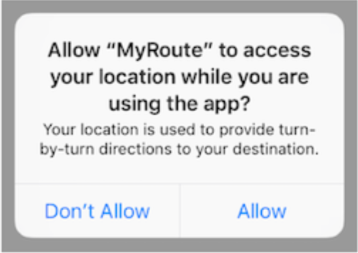
\includegraphics[width=0.5\textwidth]{image45.png}
\caption {Example of permission request message}
\label {fig02}
\end{figure}
	O objetivo de verificar o ficheiro é poder ler a justificação do uso da permissão por parte da aplicação como se pode ver na imagem abaixo.
\begin{figure}[H]
\centering
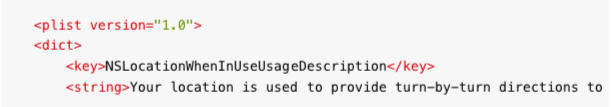
\includegraphics[width=\textwidth]{image46.png}
\caption {Example of permission request with justification}
\label {fig02}
\end{figure} 

\item \textit{Ficheiro de permissões do código da aplicação}\par
	\hfill\par

	Visualizar este ficheiro serve unicamente para verificar que a aplicação não pede permissões demasiado elevadas para o que tem de fazer permitindo assim fugas de dados.
	Na imagem abaixo podemos ver o exemplo da permissão pedida pela aplicação Telegram (aplicaçãolication-groups). Esta aplicação passa no teste por não pedir permissões adicionais, visto que não tem necessidade destas.

\begin{figure}[H]
\centering
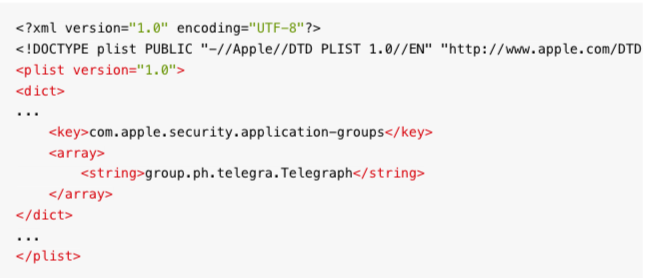
\includegraphics[width=\textwidth]{image47.png}
\caption {Example of Telegram's permission request}
\label {fig02}
\end{figure}

\item \textit{Permissões incluidas nos ficheiros binarios compilados}\par
\hfill\par
	Mais uma vez vamos procurar por permissões.
	Podemos usar a aplicação radare2 (com -qc para correr o comando e sair sem deixar registos) para procurar em todas as strings dos ficheiros binario por \textit{PropertyList} como podemos ver no exemplo abaixo.

\begin{figure}[H]
\centering
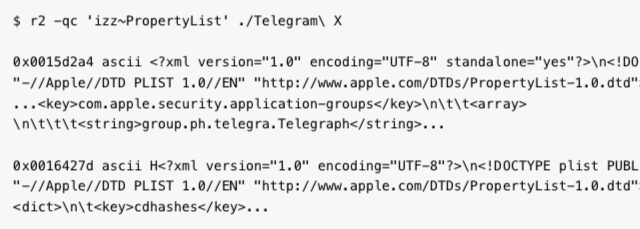
\includegraphics[width=\textwidth]{image48.png}
\caption {Result of searching for PropertyList with radare2}
\label {fig02}
\end{figure}

\item \textit{Inspeção do código fonte}\par
\hfill\par
	Esta inspeção tem de ser feita para verificar se as permissões são usadas corretamente. Assim as recomendações são:\par
	\hfill\par
	\begin{itemize}
		\item Verificar se as strings que explicam a razão pela qual a aplicação precisa da permissão e a forma como a aplicação usa essa permissão são compatíveis.\par
		\hfill\par
		\item Verificar que as permissões concedidas não são usadas para divulgamento de dados pessoais.
	\end{itemize}
\end{itemize}



\subsubsection{Testar Exposição de Dados Sensiveis através de Funcionalidades IPC (MSTG-PLATFORM-4)}
\hfill\par
\hfill\par

Durante a implementação de uma aplicação os desenvolvedores podem usar técnicas tradicionais para o IPC (como ficheiros ou sockets partilhadas), as funcionalidades do IPC para aplicações devem ser usadas visto serem muto mais seguras para não haver comprometimento de dados.\par
\hfill\par

Testar um link universal requer os seguintes passos:
\begin{enumerate}

\item \textit{Verificar as permissões do dominio associado}\par
\hfill\par
	Links universais requerem que o desenvolvedor adicione as permissões dos dominios associados numa lista de dominios que a aplicação suporte.
	Podemos usar o Xcode para verificar isto. Basta ir a \textit{Capabilities} e procurar por \textit{Associated Domains}. Em baixo mostra-se um exemplo com recurso à inspeção da aplicação Telegram.

\begin{figure}[H]
\centering
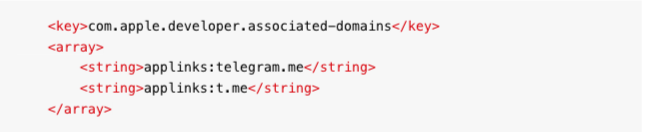
\includegraphics[width=\textwidth]{image49.png}
\caption {Example of domain permission request for universal link usage}
\label {fig02}
\end{figure}

\item \textit{Obter o ficheiro de associação no site da Apple}\par
\hfill\par

	Este ficheiro tem de ser acessivel por HTTPS sem redirecionamentos em \textit{https://<domain>/.well-known/aplicaçãole-aplicação-site-assosiation}.

	Se tudo correr bem o site verificará por nós que o link é seguro e apresentará um relatório semelhante ao mostrado.

\begin{figure}[H]
\centering
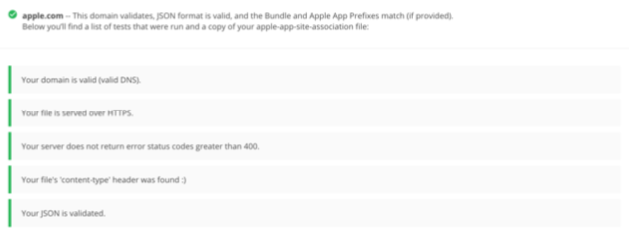
\includegraphics[width=\textwidth]{image50.png}
\caption {Safe link verifyed}
\label {fig02}
\end{figure}
	

\item \textit{Verificar o método de recepção do link}\par
\hfill\par

	Para receber o link e trata-lo de forma apropriada a aplicação tem de implementar a \textit{aplicaçãolication:continueUserActivity:restorationHandler:}. Devemos portanto procurar este método para garantir que a aplicação passa o teste.\par

	Adicionalmente, quando a aplicação usar o método \textit{openURL:options:completionHandler:} para abrir o link universal devemos verificar se o esquema da página URL é  HTTP or HTTPS. Caso nã seja, se não for lançada uma excepção a aplicação falha o teste.\par
\hfill\par

\item \textit{Verificar o método de processamento de dados}\par
\hfill\par

	Devemos verificar como são validados os dados recebidos visto que uma má verificação fornece um vetor de ataque a terçeiros. Assim todos os parâmetros fornecidos no URL não devem ser aceites sem antes serem validados.  
	A API NSURLComponents pode ser usada para verificar e manipular os componentes do URL.
	Por fim deve ser verificado que as ações requeridas pelo URL não expõem dados sensíveis.\par
\hfill\par


\item \textit{Verificar se a aplicação está a usar os links universais de outra aplicação}\par
\hfill\par

	Uma aplicação pode utilizar links de outra aplicação para transferir informação ou desencadiar alguma ação especifica, neste caso devemos garantir que não há vazamento de informação.
	Podemos para isso procurar o método \textit{openURL:options:completionHandler:} e verificar os dados manipulados.
	Em baixo temos um exemplo do que foi descrito em cima. Para este exemplo usamos o rabin2 para procurar nos ficheiros binários da aplicação.\par

\begin{figure}[H]
\centering
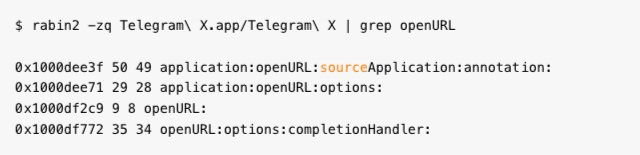
\includegraphics[width=\textwidth]{image51.png}
\caption {Result of searching for \textit{openURL:options:completionHandler:} with rabin2}
\label {fig02}
\end{figure}

	Note-se que a aplicação adapta o link para HTTPS antes de o usar e como só usa o URL caso este seja um link universal válido e só o abre caso haja uma aplicação capaz de o abrir.\par

	Como esperado o método \textit{openURL:options:completionHandler:} está implementado. Agora basta-nos garantir que dados sensíveis não são trocados entre as aplicações.\par

	Para imprimir os dados tansmitidos vamos usar o comando:
	\begin{lstlisting}[basicstyle=\small,]
 $ xcrun swift-demangle S10TelegramUI15openExternalUrl7account7
 context3url05for18applicationContext20navigationController12di
 smissInputy0A4Core7AccountC_AA1412PresentationK0CAA0a11Applica
 tionM0C7Display010NavigationO0CSgyyctF
	 \end{lstlisting}
	 Este comando apenas imprime o método \textit{TelegramUI.openExternalUrl} sem os parâmetros que lhe são passados, para que imprima mais do que isso temos de fazer alguns ajustes.\par
\hfill\par

	Primeiro vamos imprimir os parâmetros passados, alterando o ficheiro stub com se vê na imagem e o respetivo resultado de voltar a correr o comando anterior.

\begin{figure}[H]
\centering
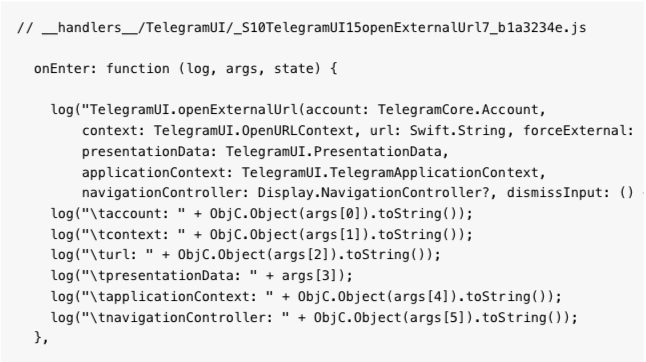
\includegraphics[width=\textwidth]{image52.png}
\caption {Code to print the parameters passed to \textit{TelegramUI.openExternalUrl}}
\label {fig02}
\end{figure}

\begin{figure}[H]
\centering
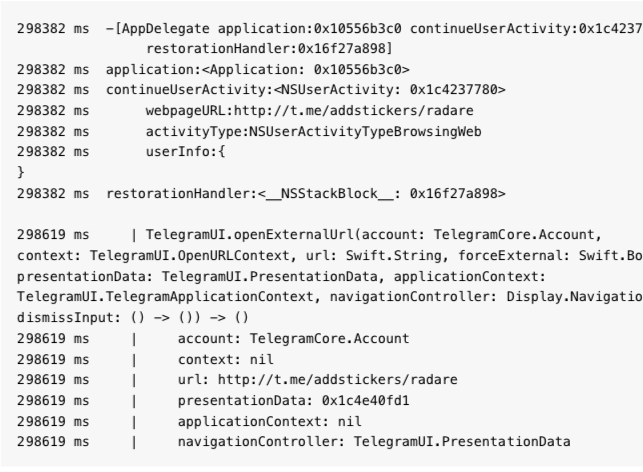
\includegraphics[width=\textwidth]{image53.png}
\caption {Parameters passed to \textit{TelegramUI.openExternalUrl}}
\label {fig02}
\end{figure}

		Aqui podemos observar que de facto o Telegram chama o método "aplicaçãolication:continueUserActivity:restorationHandler:" como esperado e que apenas trata o URL sem o abrir, chamando o \textit{TelegramUI.openExternalUrl} para isso.\par
\hfill\par

	Agora que confirmamos que o Telegram está a aplicar os métodos corretamente falta ver se temos dados sensíveis a serem trocados entre aplicações. Para isso, basta adicionar ao ficheiro stub o seguinte código: "log("userInfo:" + ObjC.Object(args[3]).userInfo().toString())". Este código  permite aceder à propriedade userInfo a partir do objeto continueUserInfo e como consequência imprime todos os dados trocados nos quais podemos verificar se existem ficheiros sensíveis.
	Na imagem seguinte vemos que não há dados sensíveis a serem passados.
	
\begin{figure}[H]
\centering
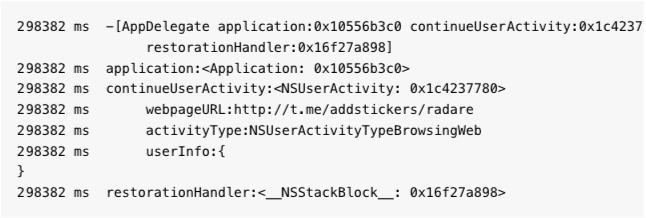
\includegraphics[width=\textwidth]{image54.png}
\caption {Print proving the safe implementation of Telegram}
\label {fig02}
\end{figure}
\end{enumerate}




\subsection{App Extensions}
\hfill\par
Para podermos analisar quais os testes a fazer temos primeiro de compreender o que são as extensões e como interagem com as aplicações.

Dependendo da tarefa, a extensão da aplicação vai ter um tipo especifico (apenas 1), o chamado ponto de extensão. Alguns exemplos são:
\begin{itemize}
\item \textit{Teclado personalizado:} substitui o teclado por um teclado personalizado para usar em todas as aplicaçãos.\par
\hfill\par

\item \textit{Partilha:} postagem para um site ou partilha de conteudos com terceiros.\par
\hfill\par

\item \textit{Hoje:} conhecidos como \textit{widgets}, oferecem conteudo ou realizam tarefas rápidas no centro de notificações.
\end{itemize}
A forma de interação com outras aplicações também pode variar:
\begin{itemize}
\item \textit{App extension:} É a extensão confinada dentro de uma aplicação. As aplicações de terceiros usam esta extensão.\par
\hfill\par

\item \textit{Host aplicação:} Trata-se da aplicação de terceiros que usa a extensão de outra aplicação.\par
\hfill\par

\item \textit{Containing aplicação:} Trata-se da aplicação que contem a extensão da aplicação instalada nela. \par
\hfill\par
\end{itemize}
Para melhor se percecionar a interação entre aplicações apresenta-se a imagem seguinte.

\begin{figure}[H]
\centering
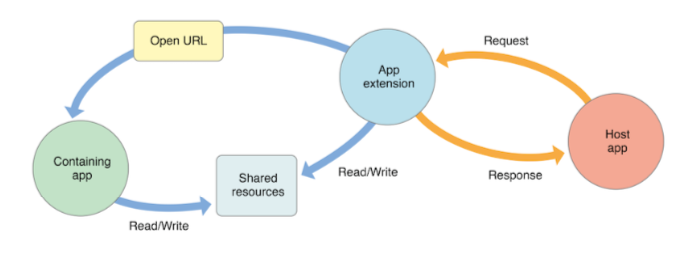
\includegraphics[width=\textwidth]{image55.png}
\caption {Aplication's shared URL implementation}
\label {fig02}
\end{figure}



\subsubsection{Determinar Exposição de Métodos Nativos através de WebViews (MSTG-PLATFORM-7)}
\hfill\par
\hfill\par

Desde o iOS a Apple introduziu APIs que permitem a comunicação entre o JavaScript na página web e o Swift ou Objective-C.
Se as APIs forem usadas de forma descuidada funcionalidades podem ser expostas através de ataques de Cross-Site Scripting.\par

Vamos então testar a UIWebView do JavaScript. Para a testarmos temos de compreender que há 2 formas fundamentais para a comunicação do JavaScript:
\begin{itemize}
	\item\textit{JSContext:} Quando é atribuido um identificador a um bloco Swift ou Objective-C num contexto JSContext, o bloco é envolto em uma função JavaScript.  \par
\hfill\par

	\item\textit{JSExport protocol:} métodos de instancia e de classes declarados no JSExport são mapeados para objetos JavaScript globais. Modificações aos objetos JavaScript são refletidas no ambiente nativo. \par
\hfill\par
\end{itemize}

Devemos portanto verificar o código que resulta do mapeamento para o JSContext para ver que funcionalidades são expostas para garantir que dados sensíveis não podem ser acedidos e expostos na WebView. \par
\hfill\par
Em Objective-C o JSContext associado a uma 	UIwebView pode-se obter com o comando:
\begin{lstlisting}[basicstyle=\small,]
[webView valueForKeyPath:@"documentView.webView.mainFrame.javaScriptContext"]
\end{lstlisting}


Para testarmos as funções devemos produzir código JavaScript para injetar num ficheiro que a aplicação utilize. Podem ser aplicadas várias técnicas para realizar isto. Vamos apresentar duas:
\begin{enumerate}

\item Se algum do conteúdo for carregado de forma insegura da internet por HTTP, podemos tentar implementar um ataque man-in-the-middle onde fornecemos o nosso código. \par
\hfill\par

\item Podemos realizar uma injeção do código ao usar frameworks como a Frida e as funções de avaliação do javaScript correspondentes a cada WebView:
	\begin{enumerate}
		\item Usar "stringByEvaluatingJavaScriptFromString:" para a UIWebView \par
\hfill\par
		\item Usar "evaluateJavaScript:completionHandler:" para a WKWebView
	\end{enumerate}
\end{enumerate}
Para efeitos de demonstração foi usada uma aplicação chamada "where's My Browser?", que fornece um serviço de calculadora web e que possui um método que, quando chamado, devolve um segredo (informação sensivel).\par
\hfill\par
Para expor o segredo da aplicação "where's My Browser?" podemos usar uma das técnicas mencionadas para injetar o seguinte código:

\begin{lstlisting}[basicstyle=\small,]
function javascriptBridgeCallBack(name, value) {
	  document.getElementById("result").innerHTML=value;
};

window.webkit.messageHandlers.javaScriptBridge.postMessage(["getSecret"]);
\end{lstlisting}
O resultado pode ser visto na imagem seguinte.

\begin{figure}[H]
\centering
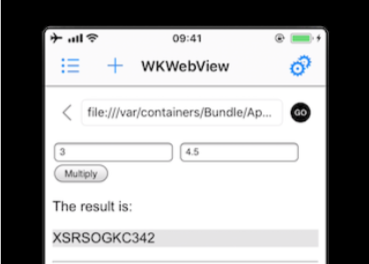
\includegraphics[width=0.5\textwidth]{image56.png}
\caption {Leaked Secret through javaScript code injection}
\label {fig02}
\end{figure}


\subsubsection{Testar Updates Forçados (MSTG-ARCH-9)}
\hfill\par
\hfill\par

Este teste tem por base a realização de updates. Como a Apple ainda não fornece uma API para automatizar o processo de atualização de aplicações os desenvolvedores terão de o programar.\par
\hfill\par

A primeira coisa a ser verificada é a presença de um mecanismo de atualização. Sem este os utilizadores não serão forçados a atualizar a aplicação.\par
Caso haja o dito mecanismo temos de verificar se este força a atualizar para "always latest". Temos também de verificar que de cada vez que se inicia a aplicação, esta passa pelo mecanismo de update para garantir que o mecanismo não pode ser ultrapassado.\par
\hfill\par

Para testar o mecanismo devemos tentar instalar uma versão da aplicação que tenha uma vulnerabilidade. De seguida devemos iniciar a aplicação e verificar se esta corre ou se nos obriga a atualizar. Se uma janela de atualização for mostrada temos de verificar se fechando-a conseguimos continuar a correr a aplicação e, caso esta continue a correr, se o backend está preparado para não nos permitir aproveitar a vulnerabilidade bloqueando-nos o acesso enquanto a aplicação não for atualizada.\par

Se todas as tentativas para explorar a vulnerabilidade falharem a aplicação foi bem sucedida.

